\documentclass[conf]{new-aiaa}
%\documentclass[journal]{new-aiaa} for journal papers
\usepackage[utf8]{inputenc}

\usepackage{graphicx}
\usepackage{amsmath}
\usepackage[version=4]{mhchem}
\usepackage{siunitx}
\usepackage{longtable,tabularx}
\usepackage{tikz}
\usepackage{pgfplots}
\pgfplotsset{compat=1.18}
\setlength\LTleft{0pt} 

\usetikzlibrary{shapes.geometric, arrows.meta, positioning, calc}

\title{Label-Free UAV Intrusion Detection via Multi-Manifold Persistent Homology}

\author{Oliver Liu\footnote{Former Undergraduate Student, Department of Computer Science, Baylor University; current affiliation: Software Engineering Associate, Capital One, Dallas, TX.}, 
Natnael Negash, Ph.D.\footnote{Postdoctoral Research Associate, Department of Mechanical Engineering, Advanced Vehicle Intelligence and Autonomy (AVIA) Laboratory, Baylor University.}, 
and Liang Sun, Ph.D.\footnote{Associate Professor, Department of Mechanical Engineering; Director, Advanced Vehicle Intelligence and Autonomy (AVIA) Laboratory, Baylor University; AIAA Associate Fellow.}}
\affil{Baylor University, Waco, TX 76798}

\begin{document}

\maketitle

\begin{abstract}
Unmanned aerial vehicle (UAV) swarms are now central to intelligence, surveillance, and reconnaissance, but methods for detecting attacks on their networks have not kept pace with adversary capabilities. Existing machine-learning-based intrusion detectors for UAV networks rely on supervised classifiers that exhibit substantial performance degradation under distribution shift and assume access to labeled adversarial training data. We apply persistent homology to UAV swarm intrusion detection on the UAVIDS-2025 benchmark. Following the functional categorization in the dataset's source paper, we partition each network flow into three pairwise-disjoint subspaces (Connection, Traffic Volume, and Performance) and compute Wasserstein-2 distances from per-flow persistence diagrams to a reference cloud of normal traffic. The resulting detector requires no exposure to attack labels at any stage of calibration. Across three random seeds, a label-free binary detector restricted to the Traffic Volume and Performance subspaces achieves an area under the receiver operating characteristic curve of $0.86 \pm 0.00$, and per-attack one-versus-rest attribution AUCs range from $0.74$ to $0.87$ on the subspace where each of four attack classes produces its strongest signal. Three of four per-attack attributions agree with the feature-level signature predictions in the source paper. The single divergence, Sybil attacks manifesting on the Traffic Volume subspace rather than the predicted Connection subspace, we discuss as a hypothesis about what topological analysis reveals beyond feature-level inspection. We position the method as a complement to supervised classification: supervised baselines achieve higher classification accuracy, while our detector provides functional-subsystem-level attribution without requiring labeled adversary data. The full manuscript will compare per-flow and time-windowed variants of the method at matched compute budgets and characterize onboard latency for UAV deployment.
\end{abstract}

\section{Introduction}

% Motivating the work: what is happening in the world?
\lettrine{U}{nmanned} aerial vehicle (UAV) swarms have become operationally central to modern intelligence, surveillance, and reconnaissance (ISR). The 2022-2025 conflict in Ukraine has demonstrated the scale of this shift. Nearly four thousand HX-2 Karma autonomous UAVs from Helsing were committed to Ukrainian forces in 2024 \cite{Bendett}. These swarm-capable drones are described as immune to electronic warfare, and are designed to operate without continuous communication to a master node or ground operator \cite{Helsing}. The 2025 India-Pakistan border conflict saw autonomous ISR swarms used as a force multiplier, providing continuity in tactical decision-making during the most serious exchange between the two nuclear powers in decades \cite{Sareen}. The United States Department of War has correspondingly accelerated its investment in drone swarm capabilities, with the 2026 ``Crucible'' demonstration event requiring autonomous completion of end-to-end ISR mission sets by swarms of at least four UAVs in simultaneous operation \cite{Harper}.

% There is a gap in the real world defensive systems for UAV swarm security 
With UAV swarm deployment accelerating across major military powers \cite{Bendett, Sareen, Harper}, their attack surface that allows adversarial exploitation has correspondingly increased \cite{Rugo}. Gaps exist in current defensive techniques against electronic warfare and offensive cyber operations that target UAV swarm networks. Computational cost is believed to be the bottleneck on expanding security from policy-based countermeasures to applicable real-world systems. Limited resources, endpoint monitoring tools lacking commercial availability, and variable environments without fixed topology are cited as factors that hamper UAV swarm intrusion detection systems \cite{Rugo}.

% The gap is against THESE ATTACKS, and due to THESE REASONS
Specific threat vectors for which current detection methods are not well-suited include synchronization attacks, beam-forming interference, and command-link compromise \cite{Cevik}. This problem is exacerbated because machine-learning based approaches to network intrusion detection systems are susceptible to adversarial attacks and distribution shifts \cite{Wang}. Meanwhile, the lack of clean, labeled datasets that contain adversarial perturbation is rarely available \cite{KacemBenjamin}, further hindering developments in robustness for UAV swarm security systems.

In this study, persistent homology is applied to the problem of intrusion detection in UAV swarms using the UAVIDS-2025 benchmark dataset \cite{Zeng}. Consistent with the functional categorization introduced in the source paper, each network flow feature vector is decomposed into three pairwise-disjoint subspaces: Connection (C2), Traffic Volume (Network), and Performance (Physical). Persistent homology is then computed independently within each subspace to characterize the underlying topological structure of the corresponding flow representation. To quantify anomalous behavior, the Wasserstein-2 distance between each flow’s persistence diagram and a reference distribution constructed from normal traffic is used to define a topology-based anomaly score. Notably, the detection framework is calibrated exclusively on benign traffic and does not rely on attack labels at any stage.
%In this work, we apply persistent homology to UAV swarm intrusion detection on the UAVIDS-2025 benchmark \cite{Zeng}. Following the functional categorization in the dataset's source paper, we partition each network flow's feature vector into three pairwise-disjoint subspaces: Connection (C2), Traffic Volume (Network), and Performance (Physical). We compute persistence diagrams independently within each subspace. Per-flow Wasserstein-2 distances to a reference cloud of normal traffic yield an anomaly score. The detector uses no attack labels at any stage of calibration.

We find that each of the four attack classes manifests its strongest signal on a specific subspace, and the attribution is reproducible across three independent random seeds. A label-free binary detector restricted to the Network and Physical subspaces achieves AUC of $0.86 \pm 0.00$. Three of four per-attack attributions agree with the feature-level signature predictions in the source paper. The one divergence, Sybil attacks manifesting on the network rather than the predicted Connection subspace, we discuss as a hypothesis about what topological analysis reveals beyond feature-level inspection.

This extended abstract addresses the following research questions:
\begin{enumerate}
    \item Do distinct attack classes in UAVIDS-2025 produce topologically distinguishable signatures on a per-manifold basis, and if so, which manifold is dominant for each attack class?
    \item Can label-free anomaly detection, calibrated using only normal-traffic samples, achieve usable binary area under the receiver operating characteristic curve (AUC) on UAVIDS-2025 without observing attack labels at any stage?
    \item Do the empirically observed per-manifold attack signatures align with the feature-level predictions in the UAVIDS-2025 source paper, and where they diverge, what does the divergence indicate?
\end{enumerate}

The remainder of the paper is organized as follows. Section II positions this work within prior research on UAV intrusion detection, topological data analysis for cybersecurity, and multi-manifold flow decomposition. Section III presents the methodology, Section IV reports the results, and Section V discusses the limitations and outlines the deliverables targeted for the full manuscript.

\section{Background and Related Work}

This section situates our contribution within three streams of prior work: UAV-specific intrusion detection (Section II.A), persistent homology applied to cybersecurity (Section II.B), and multi-manifold decompositions of network flow data (Section II.C).

\subsection{UAV Swarm Intrusion Detection}

Network intrusion detection for UAV swarms has been pursued predominantly through supervised machine learning. Zeng et al. \cite{Zeng} introduced UAVIDS-2025, a benchmark of 122,171 simulated UDP flow records spanning four attack classes (Blackhole, Wormhole, Sybil, Flooding) and Normal Traffic, and reported supervised classification accuracies exceeding $96\%$ for Random Forest baselines. Two recent surveys identify structural limitations of this supervised paradigm. Wang et al. \cite{Wang} document that ML-based intrusion detectors evaluated outside their training distribution exhibit an average AUC degradation of $30.45\%$, framing robustness rather than accuracy as the binding constraint for real-world deployment. Kacem and Benjamin \cite{KacemBenjamin}, in a survey of 62 studies on AI methods for UAV cybersecurity, find that robustness is the least-covered security property in the UAV-specific literature and that nearly all reviewed studies report results on a single dataset under stationary-distribution assumptions.

Methodological responses to these limitations have begun to appear. Mughal et al. \cite{Mughal} propose a Graph Neural Network architecture that exploits the spatial structure of UAV swarm communication graphs to generalize across varying network topologies, addressing the topology-variation case of the distribution-shift problem. Our work is methodologically distinct: rather than modeling the communication graph between UAVs, we apply algebraic topology to the geometric structure of per-flow feature vectors, addressing the label-availability case of the same broader problem. Both directions respond to the structural limitations identified by Wang et al. \cite{Wang} and Kacem and Benjamin \cite{KacemBenjamin}.

\subsection{Persistent Homology for Cybersecurity}

Persistent homology is a topological data analysis technique that summarizes the multi-scale shape of a point cloud as a barcode \cite{Ghrist}: a collection of intervals each representing the lifetime of a topological feature (connected component, loop, or higher-dimensional void) across a range of geometric scales. Davies \cite{Davies} argues that the global structure of cybersecurity data is particularly well suited to topological analysis because malicious behavior is often characterized by patterns coordinated across many observations rather than localized to any single observation. Bruillard et al. \cite{Bruillard} demonstrated this empirically in the network intrusion setting: by computing Wasserstein distances between persistence diagrams of time-windowed NetFlow data and a normal-traffic baseline, they detected DDoS and port-scan attacks without exposure to attack labels. Subsequent reviews \cite{Davies, Eroglu} confirm anomaly detection and traffic analysis as established applications of persistent homology in cybersecurity contexts.

\subsection{Multi-Manifold Decomposition of Flow Data}

The decomposition of network flows into functional subsystems is an established practice in network traffic analysis, where features describing addressing, volume, and link performance encode different aspects of network behavior. Zeng et al. \cite{Zeng} explicitly organize the UAVIDS-2025 feature set into three such functional categories (Connection, Traffic Volume, Performance) and predict per-attack signature features within each category. We are not aware of prior work that applies persistent homology to UAV swarm intrusion detection, nor that evaluates topological analysis on a functional decomposition of UAV flow data. Our contribution lies in combining the multi-manifold decomposition with per-manifold persistent homology to produce per-attack manifold attribution, an output that supervised classification on the same features does not produce.

\section{Methodology}

We apply persistent homology to UAV network flows by decomposing each flow's feature vector into three functional subsystems, computing per-flow Vietoris-Rips persistence diagrams relative to a reference cloud of normal traffic, and measuring the Wasserstein-2 distance to a baseline barcode as the anomaly score. The pipeline is illustrated in Fig.~\ref{fig:pipeline}.

\begin{figure}[h]
\centering
\resizebox{\columnwidth}{!}{\definecolor{nodeGray}{RGB}{180,180,180}
\definecolor{nodeOrange}{RGB}{200,155,80}
\definecolor{nodeViolet}{RGB}{160,130,210}
\definecolor{nodeTeal}{RGB}{90,175,160}
\definecolor{nodeSalmon}{RGB}{220,150,130}
\definecolor{labelGray}{RGB}{140,140,140}

\begin{tikzpicture}[
    box/.style={
        rectangle, rounded corners=4pt,
        minimum width=2.8cm, minimum height=1.1cm,
        align=center, font=\sffamily\small,
        text=white, inner sep=6pt
    },
    arr/.style={
        -{Latex[length=2.5mm, width=2mm]},
        line width=0.8pt, color=nodeGray!80
    },
    w2label/.style={font=\sffamily\small, color=labelGray}
]

\node[box, fill=nodeGray!70, text=black!80] (uav)
    {\textbf{UAV flow}\\[2pt] 21 features};

\node[box, fill=nodeOrange, right=1.6cm of uav] (partition)
    {\textbf{Partition}\\[2pt] Per Zeng et al.};

\node[box, fill=nodeViolet, right=2.2cm of partition, yshift=2.0cm] (c2)
    {\textbf{C2 manifold}\\[2pt] 7 features, sparse VR};

\node[box, fill=nodeTeal, right=2.2cm of partition] (net)
    {\textbf{Network manifold}\\[2pt] 10 features, sparse VR};

\node[box, fill=nodeSalmon, right=2.2cm of partition, yshift=-2.0cm] (phy)
    {\textbf{Physical manifold}\\[2pt] 5 features, exact VR};

\node[box, fill=nodeGray!70, text=black!80, right=2.4cm of net] (anomaly)
    {\textbf{Anomaly score}\\[2pt] Sum + threshold};

\draw[arr] (uav.east) -- (partition.west);
\draw[arr] (partition.east) -- ++(0.6,0) |- (c2.west);
\draw[arr] (partition.east) -- ++(0.6,0) |- (net.west);
\draw[arr] (partition.east) -- ++(0.6,0) |- (phy.west);

\draw[arr] (c2.east)  -- ++(0.5,0) |-
    node[w2label, pos=0.25, above right=0pt and 0pt] {$W_2$}
    (anomaly.north west |- anomaly.west) -- (anomaly.west);

\draw[arr] (net.east) --
    node[w2label, above, pos=0.5] {$W_2$}
    (anomaly.west);

\draw[arr] (phy.east) -- ++(0.5,0) |-
    node[w2label, pos=0.25, below right=0pt and 0pt] {$W_2$}
    (anomaly.south west |- anomaly.west) -- (anomaly.west);

\end{tikzpicture}}
\caption{Multi-manifold persistent homology pipeline. Each UAV network flow is partitioned into three functional subspaces. A Vietoris-Rips persistence diagram is computed for each manifold using a 500-point reference cloud of Normal Traffic. The Wasserstein-2 distance from each diagram to a manifold-specific baseline barcode yields a per-manifold anomaly score, which is then summed for the combined detector.}
\label{fig:pipeline}
\end{figure}

\subsection{Dataset}

We evaluate on UAVIDS-2025 \cite{Zeng}, a publicly available benchmark of 122,171 UDP flow records collected from simulated UAV swarm network traffic. Each flow record contains 23 attributes spanning addressing, traffic volume, and link performance metrics. The dataset contains five classes: Normal Traffic (26,172 flows) and four attack classes, namely Blackhole (26,110), Wormhole (26,086), Sybil (24,077), and Flooding (19,726). We use a stratified 70/15/15 train/validation/test split, yielding 85,519 training flows, 18,326 validation flows, and 18,326 test flows.

\subsection{Three-Manifold Functional Decomposition}

We partition the 21 retained flow features (dropping FlowID, an index without semantic content, and Protocol, which is constant across all flows) into three pairwise-disjoint subspaces. This partition follows the functional categorization established by Zeng et al. \cite{Zeng} in the UAVIDS-2025 source paper, where the dataset's 23 features are organized into three categories (Connection, Traffic Volume, and Performance) based on the functional role each feature plays in characterizing network behavior. We retain this categorization directly to preserve consistency with the dataset's design intent. The three manifolds, named C2, Network, and Physical for brevity, are as follows:

\begin{itemize}
    \item \textbf{C2 (Connection):} 5 features after dropping FlowID and Protocol. 7 features after preprocessing, comprising last-octet integer encoding of SrcAddr and DstAddr, one-hot indicators for the two observed ports (9 and 654) on each of SrcPort and DstPort, and FlowDuration.
    \item \textbf{Network (Traffic Volume):} 10 features, comprising TxPackets, RxPackets, LostPackets, TxBytes, RxBytes, TxPacketRate, RxPacketRate, TxByteRate, RxByteRate, and MeanPacketSize.
    \item \textbf{Physical (Performance):} 5 features, comprising MeanDelay, MeanJitter, Throughput, PacketDropRate, and AverageHopCount.
\end{itemize}

All features are standardized to a zero mean and unit variance using statistics computed on the training split only. Let $x_{i,j}$ denote the raw value of feature $j$ in flow $i$, and let $\mathcal{T}$ denote the set of training-split flow indices. For each feature $j$, we compute the training-split mean and standard deviation,

\begin{equation}
\mu_j = \frac{1}{|\mathcal{T}|} \sum_{i \in \mathcal{T}} x_{i,j}, \qquad \sigma_j = \sqrt{\frac{1}{|\mathcal{T}|} \sum_{i \in \mathcal{T}} (x_{i,j} - \mu_j)^2}.
\label{eq:scaling_stats}
\end{equation}

We then apply the transformation

\begin{equation}
z_{i,j} = \frac{x_{i,j} - \mu_j}{\sigma_j}
\label{eq:zscore}
\end{equation}

to every flow $i$ across the training, validation, and test splits, using the same $\mu_j$ and $\sigma_j$ from Eq.~\eqref{eq:scaling_stats}. The values $\mu_j$ and $\sigma_j$ are never recomputed on validation or test data, which would leak information about those splits into the preprocessing. Standardization is necessary because the raw features span several orders of magnitude (packet counts in the thousands, packet drop rates in the hundredths) and Euclidean distances would otherwise be dominated by the highest-magnitude features. The 25th-percentile pairwise-distance filtration cap reported in the next subsection is therefore in standardized units.

Our methodological contribution is not the decomposition itself but the application of persistent homology independently within each subspace. Single-manifold analyses compute topology over all features jointly and produce a single anomaly signal per flow. Our hypothesis is that different attack classes distort the topology of different functional subspaces, and that per-manifold attribution provides interpretive information that single-manifold analysis cannot.

\subsection{Reference Cloud Construction}

For each manifold, we construct a 500-point reference cloud representing normal UAV traffic. We apply k-medoids clustering \cite{Kaufman} to the Normal Traffic flows in the training split and select the 500 medoid flows as the reference cloud. K-medoids is preferred over k-means because medoids are actual observed flows rather than synthetic averages, and because using the same 500 row positions across all three manifolds preserves the correspondence between reference points across subspaces. In a deployment scenario, this reference cloud corresponds to a controlled training-flight phase during which only benign operational regimes are exercised. The design of such a training-flight protocol, including controlled environment selection, planned flight scenarios, and any simulated adversarial activity, is outside the scope of this work and is left to future investigation.

\subsection{Per-Flow Vietoris-Rips Filtration}

For each query flow $q$ and each manifold $m$, we construct a Vietoris-Rips simplicial complex on the union $P_m = \{q\} \cup R_m$, where $R_m$ is the $500$-point reference cloud for manifold $m$. The query flow is dropped into the reference cloud, and the topology of the combined $501$-point set is compared against the topology of the reference cloud alone. If the query is normal, the topology is essentially unchanged; if the query is anomalous, the query point lands in an unusual location and distorts the topology.

The Vietoris-Rips complex at scale $\epsilon$, denoted $\text{VR}(P_m, \epsilon)$, contains a $k$-simplex for every subset of $k+1$ points in $P_m$ whose pairwise Euclidean distances are all at most $\epsilon$. As $\epsilon$ grows from $0$ to $\infty$, the complex grows monotonically: at $\epsilon = 0$, only the $501$ vertices are present; at large $\epsilon$, every subset of points forms a simplex. The \emph{persistence filtration} tracks the appearance (birth) and disappearance (death) of topological features as $\epsilon$ varies, encoding the result as a barcode \cite{Ghrist}, $B_m$, in which each feature is represented as an interval $[b, d)$ from its birth scale $b$ to its death scale $d$. Long intervals correspond to robust topological features that persist across many scales; short intervals correspond to features that appear and die quickly and are typically interpreted as noise.

In principle the filtration sweeps from $0$ to $\infty$, but computation at large scales is prohibitively expensive and topologically uninformative, as every point eventually connects to every other. We therefore cap the filtration at a maximum edge length $\epsilon_{\max,m}$ determined per manifold from the reference-cloud geometry. Specifically, let $\mathcal{D}_m = \{ \|r_i - r_j\|_2 : r_i, r_j \in R_m, i < j \}$ denote the multiset of pairwise Euclidean distances in the reference cloud for manifold $m$. We set

\begin{equation}
\epsilon_{\max,m} = Q_{0.25}(\mathcal{D}_m),
\label{eq:filtration_cap}
\end{equation}

where $Q_{0.25}$ is the $25$th percentile of the distance distribution. This data-adaptive cap normalizes for the differing intrinsic scales of the three subspaces and yields $\epsilon_{\max} = 0.494$ for C2, $0.145$ for Network, and $0.333$ for Physical (in standardized units, following Eq.~\eqref{eq:zscore}). The 25th-percentile choice is consistent with the data-adaptive scale-selection approach in prior topological anomaly detection work \cite{Bruillard} and balances coverage of medium-scale topological features against computational cost.

The Vietoris-Rips complex on $n$ points can contain up to $\binom{n}{k+1}$ simplices of dimension $k$, which is intractable to enumerate for $n = 501$ and large $k$. We mitigate this in two ways. First, we cap the simplex tree \cite{BoissonnatMaria} at a maximum dimension $k_{\max}$, retaining only simplices of dimension at most $k_{\max}$ and consequently computing homology only in dimensions $H_0, H_1, \ldots, H_{k_{\max}-1}$. Second, for the higher-dimensional manifolds where the Rips complex grows rapidly, we use a sparse approximation.

For the Physical manifold (ambient dimension $5$), the exact Vietoris-Rips complex remains computationally tractable within our per-flow runtime budget. We use exact Rips with $k_{\max} = 2$, yielding barcodes in dimensions $H_0$ (connected components) and $H_1$ (loops). For the C2 (ambient dimension $7$) and Network (ambient dimension $10$) manifolds, exact construction is too expensive at scale. We use sparse Vietoris-Rips \cite{Cavanna} with sparsification parameter $\varepsilon_s = 0.5$ and $k_{\max} = 3$, yielding barcodes in $H_0$, $H_1$, and $H_2$ (voids). The sparsification parameter $\varepsilon_s$ governs the approximation quality: sparse Rips guarantees that the bottleneck distance between the sparse and exact barcodes is bounded as a function of $\varepsilon_s$, with smaller values yielding tighter approximations at higher computational cost. The value $\varepsilon_s = 0.5$ is a moderate setting consistent with similar applications in topological anomaly detection. All barcodes are computed using the GUDHI library \cite{Maria}.

\subsection{Anomaly Scoring}

The baseline barcode for each manifold is computed once from the reference cloud alone. For manifold $m$, let $B_m^{\text{ref}}$ denote the barcode obtained by applying the Vietoris-Rips construction of Section III.D to $R_m$ (without any query flow). For a given query flow $q$, let $B_{m,q}$ denote the barcode obtained from $P_m = \{q\} \cup R_m$. The anomaly score for flow $q$ on manifold $m$ is the Wasserstein-2 distance between these two barcodes, summed across homology dimensions:

\begin{equation}
s_m(q) = \sum_{k=0}^{k_{\max,m}-1} W_2\!\left( B_{m,q}^{(k)},\, B_m^{\text{ref},(k)} \right),
\label{eq:anomaly_score}
\end{equation}

where $B^{(k)}$ denotes the restriction of barcode $B$ to homology dimension $k$, and $k_{\max,m} = 3$ for C2 and Network and $k_{\max,m} = 2$ for Physical.

The Wasserstein-2 distance between two barcodes views each barcode as a set of points $(b, d)$ in $\mathbb{R}^2$ and computes the minimum-cost matching of points in one barcode to points in the other, with unmatched points on either side matched to the diagonal $\{(x, x) : x \in \mathbb{R}\}$. The cost of matching two points is the squared $L^\infty$ distance between them; the Wasserstein-2 distance is the square root of the minimum total cost over all valid matchings. We use the Wasserstein-2 form rather than Wasserstein-1 because squared cost disproportionately penalizes large displacements, which is appropriate when anomalies produce a small number of substantially displaced topological features rather than many small distributed perturbations. Wasserstein distances are computed using the Hera backend \cite{Kerber} via GUDHI \cite{Maria}.

To combine evidence across manifolds, the per-manifold anomaly scores are summed without weighting:

\begin{equation}
s(q) = \sum_{m \in \{ \text{C2, Network, Physical} \}} s_m(q).
\label{eq:combined_score}
\end{equation}

We acknowledge that the three manifolds produce distances on different scales, with raw C2 distances roughly five times larger in magnitude than Network or Physical distances. The full manuscript will report results under per-manifold Z-score normalization computed on held-out validation Normal Traffic. In this extended abstract we report the unweighted-sum results to maintain a strict separation between calibration data and evaluation data.

Threshold calibration for binary detection uses only Normal Traffic flows from the validation split. Let $\mathcal{V}_{\text{normal}}$ denote the set of Normal Traffic flow indices in the validation split. The decision threshold $\tau$ is set at the 95th percentile of the validation Normal Traffic anomaly score distribution:

\begin{equation}
\tau = Q_{0.95}\!\left( \{ s(q) : q \in \mathcal{V}_{\text{normal}} \} \right).
\label{eq:threshold}
\end{equation}

A flow $q$ is flagged as anomalous if $s(q) > \tau$. The detector therefore never observes attack labels at any stage, satisfying our label-free constraint.

\subsection{Computational Approximation}

The exact computation of Wasserstein-2 distances between persistence diagrams scales poorly with diagram size. For tractability, we report results from a confirmation probe configuration: 200 randomly sampled flows per class from the test split, with Wasserstein distances computed using Hera's approximate mode at relative error $\delta = 0.2$ and per-diagram truncation to the top $K = 50$ most persistent features. This configuration completes per seed in approximately 60 seconds on a 2021-era laptop (Apple M1 Pro, 8 cores). We verified that doubling the diagram resolution from a prior $K = 20$, $\delta = 0.5$ configuration produced consistent attack-attribution rankings, confirming that results are not artifacts of aggressive approximation. The full manuscript will report exact Wasserstein computation on the complete test set.

We evaluate across three random seeds (42, 7, 123) and report mean and standard deviation of all AUC metrics. The seed determines random sampling of the 200 per-class probe flows, k-medoids initialization, and tiebreaking inside the Wasserstein matching.

\section{Results}

We report results from the confirmation probe configuration described in Section III.F: 200 flows per class drawn from the test split, with Wasserstein-2 distances computed under sparse approximation, averaged across three random seeds (42, 7, 123). Section IV.A establishes the supervised baseline context. Section IV.B reports per-attack manifold attribution. Section IV.C reports label-free binary anomaly detection performance.

\subsection{Supervised Classifier Context}

A Random Forest classifier trained on the raw 21-feature flow vectors achieves $96.3\%$ test-set classification accuracy on UAVIDS-2025, consistent with the supervised baseline reported by Zeng et al. \cite{Zeng}. We further evaluated whether topological features extracted from per-flow persistence diagrams improve on this baseline by concatenating per-manifold persistence-image vectors with the raw features and retraining Random Forest, Logistic Regression, and Support Vector Machine classifiers. None of the resulting models improved on the raw-feature baseline. We therefore do not claim that persistent homology augments supervised classification on UAVIDS-2025, and the remainder of this section evaluates a different question: what does topology reveal that supervised classification on raw features does not?

\subsection{Per-Attack Manifold Attribution}

We evaluate per-attack manifold attribution using one-versus-rest AUC. For each attack class $c$ and each manifold $m$, we treat class $c$ as the positive class and all other classes (Normal, plus the three remaining attack classes) as the negative class, and compute the AUC using the per-manifold anomaly score $s_m(q)$ from Eq.~\eqref{eq:anomaly_score} as the ranking signal. The AUC measures the probability that a randomly chosen flow of class $c$ receives a higher anomaly score than a randomly chosen flow of any other class; values near $1.0$ indicate that manifold $m$ effectively isolates attack class $c$ from the rest of the data, while values near $0.5$ indicate no separation. We compute the AUC using \texttt{sklearn.metrics.roc\_auc\_score}.

To assess reproducibility, we repeat the full evaluation for three independently chosen random seeds (42, 7, 123), each of which determines the random sampling of 200 flows per class for the probe, the k-medoids reference cloud initialization, and tiebreaking inside the Wasserstein matching. Table~\ref{tab:per_attack_auc} reports the resulting AUC values as the per-seed arithmetic mean and standard deviation:

\begin{equation}
\overline{\text{AUC}}_{c, m} = \frac{1}{3} \sum_{i \in \{42, 7, 123\}} \text{AUC}_{c, m}^{(i)},
\label{eq:auc_mean}
\end{equation}

where $\text{AUC}_{c, m}^{(i)}$ is the one-versus-rest AUC for attack class $c$ on manifold $m$ at seed $i$. Each attack class produces its strongest signal on a specific manifold, and this attribution is reproducible across all three seeds.

\begin{table}[h]
\centering
\caption{Per-attack one-versus-rest AUC on each manifold, mean $\pm$ standard deviation across three seeds. Dominant manifold for each attack is shown in bold.}
\label{tab:per_attack_auc}
\begin{tabular}{lccc}
\hline
Attack class & C2 & Network & Physical \\
\hline
Sybil & $0.65 \pm 0.01$ & $\mathbf{0.87 \pm 0.00}$ & $0.20 \pm 0.01$ \\
Flooding & $0.60 \pm 0.03$ & $\mathbf{0.79 \pm 0.01}$ & $0.38 \pm 0.01$ \\
Blackhole & $0.46 \pm 0.02$ & $0.33 \pm 0.02$ & $\mathbf{0.79 \pm 0.02}$ \\
Wormhole & $0.54 \pm 0.03$ & $0.28 \pm 0.02$ & $\mathbf{0.74 \pm 0.01}$ \\
\hline
\end{tabular}
\end{table}

Two volumetric attacks (Sybil, Flooding) manifest most strongly on the Network manifold, with mean AUCs of $0.87$ and $0.79$ respectively. Two routing-manipulation attacks (Blackhole, Wormhole) manifest most strongly on the Physical manifold, with mean AUCs of $0.79$ and $0.74$. Standard deviations at the dominant manifold are at most $0.02$ across all four attacks, indicating the attribution is not an artifact of any individual seed.

Three of these four attributions are consistent with the feature-level signature predictions in Zeng et al. \cite{Zeng}. Zeng et al. predict that Blackhole attacks produce elevated PacketDropRate and reduced Throughput (both Physical-manifold features), that Wormhole attacks produce reduced AverageHopCount and inconsistent MeanDelay (both Physical-manifold features), and that Flooding attacks produce anomalous transmission rates and volume metrics (Network-manifold features). Our empirical attributions agree on these three.

Sybil is the single divergence. Zeng et al. predict that Sybil attacks manifest through unusual patterns in source addressing (SrcAddr, SrcPort), all of which are C2-manifold features. Our topology finds Sybil's strongest signature on the Network manifold (AUC $0.87 \pm 0.00$) rather than C2 (AUC $0.65 \pm 0.01$). One plausible interpretation is that a Sybil attacker forging multiple identities must also generate traffic from each forged identity, and the volumetric pattern of that traffic (many low-volume flows from disparate sources) is more topologically structured than the address-space distribution of the identities themselves, which in the simulated dataset are essentially uniformly distributed. We propose this hypothesis tentatively; distinguishing it from alternative explanations (e.g., a peculiarity of the UAVIDS-2025 simulation) is left to future investigation.

\subsection{Label-Free Binary Detection}

For binary normal-versus-attack detection using the threshold construction in Eq.~\eqref{eq:threshold}, the best-performing manifold subset is Network+Physical, which achieves binary AUC of $0.86 \pm 0.00$ across the three seeds (Fig.~\ref{fig:binary_auc}). Combining all three manifolds yields statistically equivalent performance ($0.86 \pm 0.03$) with substantially larger variance, indicating that the C2 manifold contributes additional noise more than additional signal at the combined-detector level. Single-manifold detection is uniformly weaker: Network alone reaches $0.76 \pm 0.02$, C2 alone $0.75 \pm 0.03$, and Physical alone $0.61 \pm 0.02$.

\begin{figure}[h]
\centering
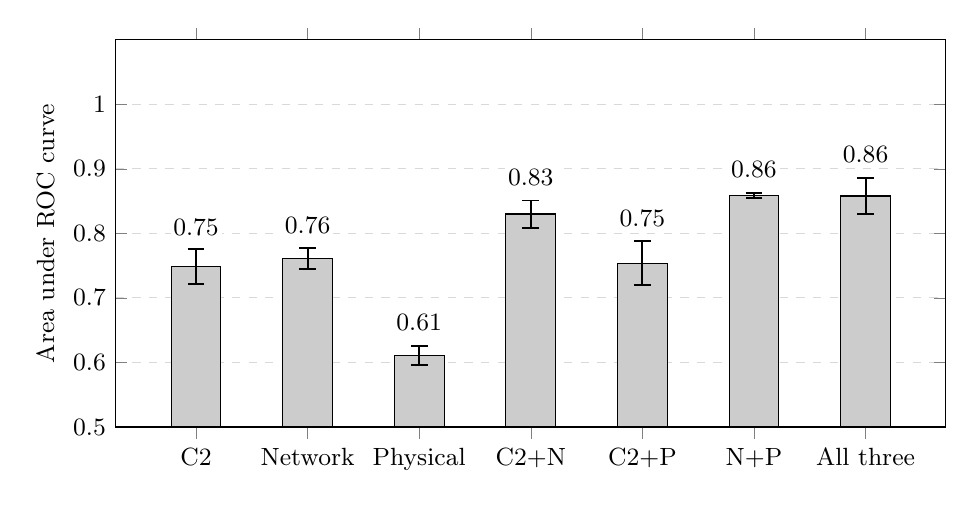
\begin{tikzpicture}
\begin{axis}[
    width=\textwidth,
    height=6.5cm,
    ybar,
    bar width=18pt,
    enlarge x limits=0.12,
    ymin=0.5, ymax=1.10,
    ylabel={Area under ROC curve},
    ylabel style={font=\small},
    symbolic x coords={C2, Network, Physical, C2+N, C2+P, N+P, All three},
    xtick=data,
    xticklabel style={font=\small, align=center},
    yticklabel style={font=\small},
    ytick={0.5,0.6,0.7,0.8,0.9,1.0},
    ymajorgrids=true,
    grid style={dashed, gray!30},
    error bars/y dir=both,
    error bars/y explicit,
    error bars/error bar style={line width=0.7pt, black},
    error bars/error mark options={rotate=90, mark size=3pt, line width=0.7pt},
]

\addplot+[
    fill=gray!40,
    draw=black,
    error bars/.cd, y dir=both, y explicit,
] coordinates {
    (C2, 0.749) +- (0, 0.027)
    (Network, 0.761) +- (0, 0.016)
    (Physical, 0.611) +- (0, 0.015)
    (C2+N, 0.830) +- (0, 0.021)
    (C2+P, 0.754) +- (0, 0.034)
    (N+P, 0.859) +- (0, 0.004)
    (All three, 0.858) +- (0, 0.028)
};

% Manual value labels placed above upper whiskers
\node[font=\small, anchor=south, fill=white, inner sep=1pt] at (axis cs:C2,0.792) {0.75};
\node[font=\small, anchor=south, fill=white, inner sep=1pt] at (axis cs:Network,0.795) {0.76};
\node[font=\small, anchor=south, fill=white, inner sep=1pt] at (axis cs:Physical,0.644) {0.61};
\node[font=\small, anchor=south, fill=white, inner sep=1pt] at (axis cs:C2+N,0.869) {0.83};
\node[font=\small, anchor=south, fill=white, inner sep=1pt] at (axis cs:C2+P,0.806) {0.75};
\node[font=\small, anchor=south, fill=white, inner sep=1pt] at (axis cs:N+P,0.881) {0.86};
\node[font=\small, anchor=south, fill=white, inner sep=1pt] at (axis cs:All three,0.904) {0.86};

\end{axis}
\end{tikzpicture}
\caption{Binary normal-versus-attack area under the ROC curve across the seven manifold subsets evaluated. Bar heights are the mean across three seeds (42, 7, 123); error bars show one standard deviation. Network+Physical (N+P) achieves the highest mean with the lowest variance; including C2 in the combined detector matches the mean but inflates the variance.}
\label{fig:binary_auc}
\end{figure}

We highlight that this detection performance is achieved without any exposure to attack labels at any stage. The reference cloud is sampled from Normal Traffic in the training split; the decision threshold is calibrated on Normal Traffic in the validation split; only the final AUC computation uses ground-truth labels on the test split for evaluation. The threshold percentile of $0.95$ on validation Normal Traffic yields a false-positive rate near $0.05$ on Normal Traffic in the test split, confirming that the threshold calibration transfers cleanly across splits.

The headline numbers position the method as a complement to supervised classification rather than a replacement. Supervised Random Forest, given a labeled training set covering all four attack classes, achieves higher classification accuracy than our detector achieves AUC. Our detector, given no attack labels at all, achieves binary detection AUC of $0.86$ and per-attack attribution AUCs of $0.74$ to $0.87$, providing functional-subsystem-level interpretation that supervised classification does not produce.

\section{Limitations and Future Work} %Manuscript Extension}

\subsection{Limitations}

\textit{Probe approximation.} Results in this extended abstract are computed under an approximation regime: 200 randomly sampled flows per class from the test split, with Wasserstein-2 distances computed via Hera's relative-error mode at $\delta = 0.2$ and per-diagram truncation to the top $K = 50$ persistent features. We verified through a confirmation probe that doubling the diagram resolution from $K = 20$, $\delta = 0.5$ to the present configuration produced consistent attack-attribution rankings, indicating that the headline findings are not artifacts of aggressive approximation. Exact Wasserstein computation on the full test set is deferred to the full manuscript.

\textit{Single-dataset evaluation.} All findings are reported on UAVIDS-2025 \cite{Zeng}, a single simulated benchmark. We make no claims about generalization to other UAV intrusion benchmarks or to real UAV network traffic, and we do not address the cross-dataset robustness limitations identified in Section II.A. Cross-benchmark evaluation is deferred to the full manuscript.

\textit{Per-manifold scale heterogeneity.} The three manifolds produce Wasserstein-2 distances on substantially different scales, with raw C2 distances roughly five times the magnitude of Network or Physical distances. In the headline configuration, per-manifold scores are summed without weighting; this is methodologically conservative because it avoids using validation data to determine per-manifold weights, but it is not the principled scaling choice. Per-manifold Z-score normalization computed on held-out validation Normal Traffic is the appropriate correction and is deferred to the full manuscript.

\textit{Hera approximation artifact on one seed.} Approximately $4.6\%$ of C2 manifold Wasserstein-2 computations on seed 123 exceeded a 5-second per-call cap and were truncated by the timeout mechanism, slightly depressing C2 anomaly scores for the affected flows on that seed. Network and Physical manifold computations completed without timeout across all three seeds. The dominant-manifold attributions reported in Section IV.B occur on Network and Physical for all four attack classes; the timeout artifact therefore does not affect the per-attack attribution finding. Variance estimates that include the C2 manifold (the C2-only, C2+Network, C2+Physical, and all-three binary AUC combinations in Fig.~\ref{fig:binary_auc}) inherit a small additional spread from this artifact and should be interpreted accordingly.

\subsection{Manuscript Extension}

The full manuscript, targeted for the December 2026 submission deadline, will extend this work along three axes.

\textit{Per-flow versus time-windowed analysis.} The methodology presented here operates per-flow, providing the maximum-resolution variant of multi-manifold persistent homology. A time-windowed variant, in which flows are aggregated into temporal windows and persistence diagrams are computed per window, reduces per-decision compute by a factor proportional to window size at the cost of attribution resolution. The full manuscript will report a direct comparison between per-flow and time-windowed regimes on UAVIDS-2025 at matched compute budgets, characterizing the tradeoff between detection latency, attribution resolution, and detection AUC. This comparison is the lead methodological contribution of the manuscript and motivates the deployment characterization that follows.

\textit{Onboard latency profiling.} Per-flow inference on the present 2021-era laptop hardware requires approximately one to three seconds per flow, consistent with periodic security audits but not with per-packet intrusion detection. The full manuscript will report onboard latency profiling on ARM-class hardware representative of typical UAV companion computers, identifying the operational regime in which time-windowed multi-manifold persistent homology is viable for in-flight deployment.

\textit{Multi-seed evaluation and methodological refinements.} The present three-seed evaluation will expand to ten seeds with bootstrap confidence intervals, addressing the variance characterization that three seeds support only at the paper-ready threshold. Per-manifold Z-score normalization on held-out validation Normal Traffic will replace the unweighted sum used here, so that all three manifolds contribute on comparable scales. The Hera approximation artifact on seed 123 will be reanalyzed under an extended per-call timeout, eliminating the localized C2-manifold artifact. Exact Wasserstein computation on the full test set will replace the probe approximation, providing definitive AUC values rather than the bounded-approximation estimates reported here.

\section{Conclusion}

We applied multi-manifold persistent homology to UAV swarm intrusion detection on the UAVIDS-2025 benchmark, decomposing each network flow into three functional subspaces and computing per-manifold anomaly scores via Wasserstein-2 distance to a reference cloud of normal traffic. The resulting detector requires no attack labels at any stage and achieves binary detection AUC of $0.86 \pm 0.00$ on the Traffic Volume and Performance subspaces. Each of four attack classes produces a reproducible signal on a specific subspace, and three of four attributions agree with the feature-level predictions in the dataset's source paper. The single divergence (Sybil attacks manifesting on Traffic Volume rather than the predicted Connection subspace) suggests that topological analysis captures structural signatures that flow-feature inspection does not.

The contribution is functional-subsystem-level attribution under label-free calibration, complementary to the higher classification accuracy of supervised baselines that require labeled adversary data. As UAV swarm deployment continues to outpace the availability of labeled attack corpora, detection methods that calibrate on normal operational data alone become operationally relevant. The full manuscript characterizes the deployment-oriented variants of this approach.

\section*{Acknowledgments}

Oliver Liu thanks co-advisors Dr. Liang Sun (Associate Professor in the Department of Mechanical Engineering and Director of the Advanced Vehicle Intelligence and Autonomy Laboratory at Baylor University, AIAA Associate Fellow) and Dr. Natnael Negash (Postdoctoral Research Associate in the Department of Mechanical Engineering at Baylor University) for their guidance throughout this research and their detailed feedback on the manuscript. This project originated in the 2026 Engineering and Computer Science Summit Research Showcase at Baylor University, where an earlier formulation of this work, titled ``Reading the Shape of an Attack: Topology-Based Intrusion Detection for Drone Swarms,'' received first place in the undergraduate category under Dr. Sun's faculty mentorship. The present extended abstract substantially refines that work and reports findings derived from subsequent experiments.

Anthropic's Claude was used during manuscript preparation to assist with drafting text, refining mathematical notation, refactoring the experiment code, and writing \LaTeX{} figures. The authors directed all substantive decisions, including the research questions, experiment design, methodology, data analysis, and conclusions. All AI-generated content was reviewed and revised by the authors before inclusion in the manuscript.

\bibliography{references}

\end{document}
